Alla olevassa sekvenssikaaviossa on havainnollistettu UML-kielellä uuden kaatosysteemin toimintaa.

\begin{figure}[h]
\begin{center}
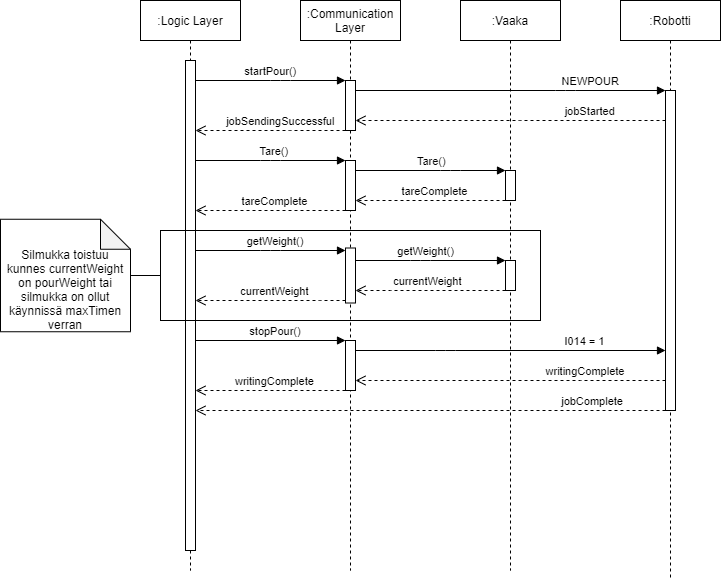
\includegraphics[scale=0.6]{img/Sequence.png}
\end{center}
\caption{Sekvenssikaavio uudesta kaatosysteemistä}
\label{fig:Sequence}
\end{figure}

Logiikka laskee halutun juoman massan kaavalla
\[pourWeight = pourAmount \cdot 10  - 27, \]
eli halutusta massasta vähennetään vaa'an hitautta kuvaava vakio 27. Hitaus johtuu muun muassa tietoliikenneyhteyden hitaudesta ja looppien sisällä olevista odotusajoista. Esimerkiksi robotin jobissa olevaa timeria tai logiikassa olevaa sleepiä nostamalla tuo vakio 27 kasvaisi. Tämä hitaus tarkoittaa sitä, että pullon suoristusliikkeen aikana tapahtuviin muuttujiin ei pystytä enää vaa'an avulla vaikuttamaan. Tämä on kuitenkin vain pieni osa koko kaatoliikettä.
